\documentclass[../notes.tex]{subfiles}

\pagestyle{main}
\renewcommand{\chaptermark}[1]{\markboth{\chaptername\ \thechapter\ (#1)}{}}

\begin{document}




\chapter{Carbocations, Carbanions, and Radicals}
\section{Problems 1, 2, and 6}
\begin{itemize}
    \item \marginnote{9/4:}Logistics.
    \begin{itemize}
        \item The list of topics is the syllabus.
        \item We'll cover everything we need to know in discussion, but we can supplement what we discuss here with our own readings.
        \begin{itemize}
            \item Mo recommends the OChem II textbook.
        \end{itemize}
        \item Students: Frank, Christina, Jasmin, Alex (senior undergrad), and Ivan.
        \item PSet 2 passed out on paper.
        \item The locked door code for 18-578 is 9344, if we ever get here before him.
        \item He'll ask us at the beginning of class which problems seem the most interesting to us.
        \item We should try every problem on the PSet before class.
        \item We'll probably put multiple problems up at the same time.
        \begin{itemize}
            \item This is a team effort to sort out the board, not one person defending their solution.
        \end{itemize}
        \item We will not get through six problems every time.
        \item These problems are basically ice breakers for discussion.
        \item He encourages us to compare notes and compare solutions, but we must try all the problems first by ourselves.
        \begin{itemize}
            \item Do not search for the solutions on Google; this takes away from the discussion.
        \end{itemize}
        \item Mo will send PSet 2 as a PDF!
        \item These examples were chosen to start because Mo wants to begin with bond dissociation energy, carbocations, carbanions, and radical chemistry.
    \end{itemize}
    \item We now begin discussing Problem 1.
    \begin{figure}[H]
        \centering
        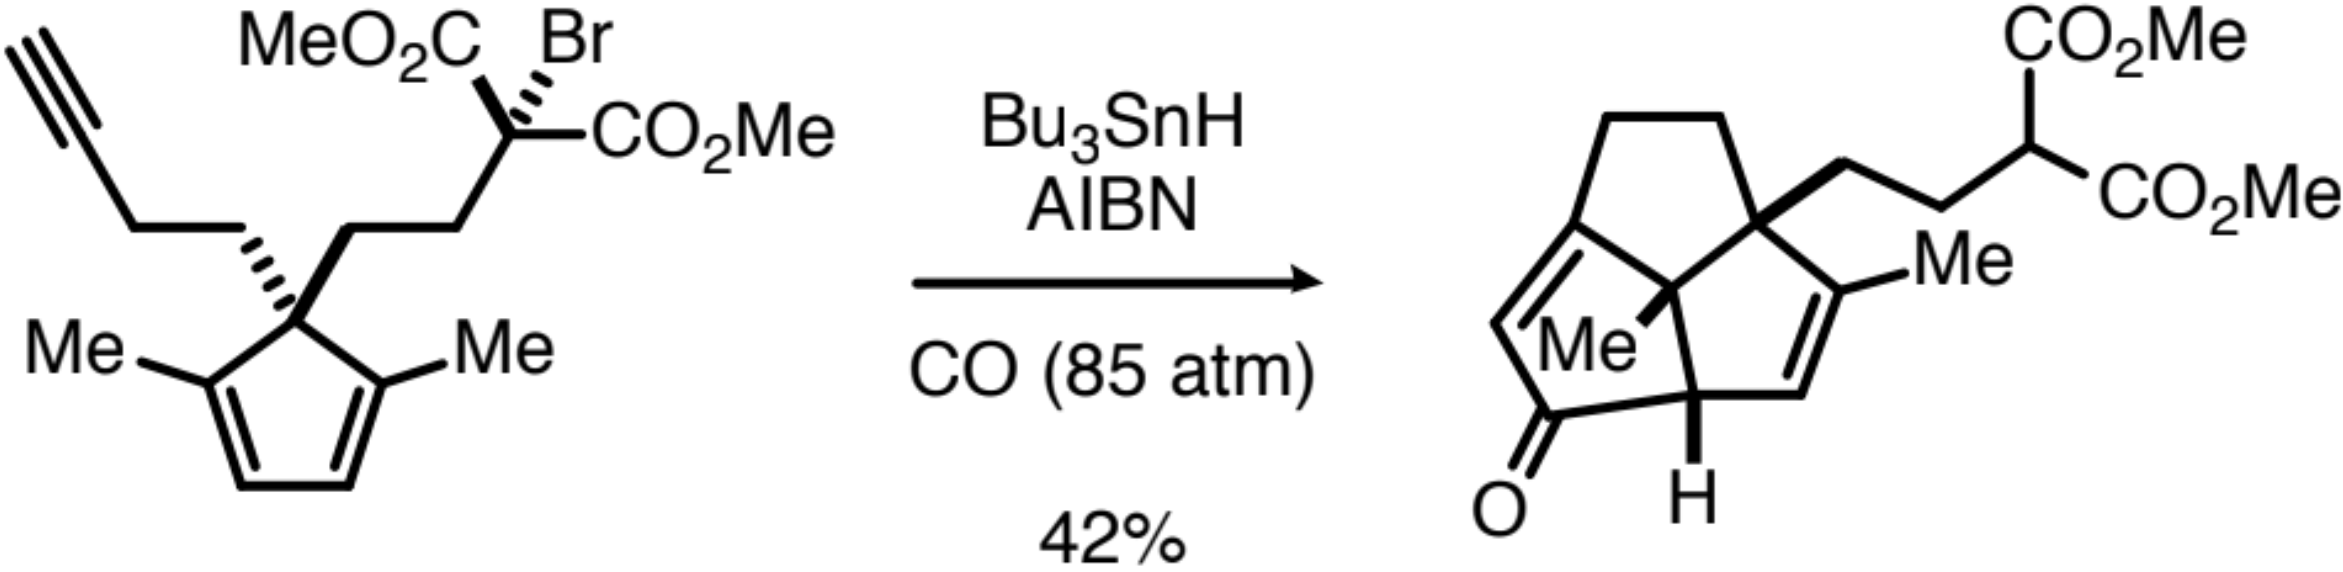
\includegraphics[width=0.55\linewidth]{PSet1Q1.png}
        \caption{PSet 1, Q1.}
        \label{fig:PSet1Q1}
    \end{figure}
    \item A \emph{key} technique for thinking about, rationalizing, and solving this problem is \textbf{bond dissociation energy} (BDE).
    \item In fact, we can apply BDE from the very beginning: AIBN's \ce{C-N} bond is the first to break because its BDE is an extremely low $\sim\SI{30}{\kilo\calorie\per\mole}$.
    \begin{itemize}
        \item Additionally, AIBN's \ce{C-N} bonds do not have to break symmetrically. Rather, one bond may break first (driven by its vibrational modes) to generate the stable tertiary carbon-centered radical \emph{and} a nitrogen radical.
        \item After some finite time (from picoseconds to much longer), the second \ce{C-N} bond will split, off-gassing \ce{N2}.
    \end{itemize}
    \item At this point, we must remember that this is a three-step radical reaction (initiation, propagation, termination), and AIBN is our initiator.
    \begin{itemize}
        \item Thus, we don't have \emph{equivalents} of AIBN to speak of, but rather a tiny amount in a sea of everything else.
    \end{itemize}
    \item Our AIBN radical is very stable, but the \ce{H-SnBu3} bond is so weak that it will still break when the two bump into each other.
    \item Indeed, BDE can justify why this bond breaks over any of the reactant \ce{C-H}'s.
    \begin{itemize}
        \item \ce{H3C-H} is $\SI{100}{\kilo\calorie\per\mole}$.
        \item \ce{HR2C-H} is $\sim\SI{90}{\kilo\calorie\per\mole}$.
        \item Tributyl tin hydride BDE is a whopping $\sim\SI{73}{\kilo\calorie\per\mole}$.
        \item Know BDEs!! \href{https://en.wikipedia.org/wiki/Carbon%E2%80%93hydrogen_bond#Reactions}{Here}'s a great resource for \ce{C-H} bonds on Wikipedia.
    \end{itemize}
    \item The \ce{*SnBu3} radical is halophilic, and does indeed head straight for the bromine to form a resonance-stabilized radical on the reactant.
    \begin{itemize}
        \item A typical \ce{C-Br} BDE is $\SI{68}{\kilo\calorie\per\mole}$.
        \item Why does AIBN pick off the \ce{H-SnBu3} over the bromine, then??
        \begin{itemize}
            \item Alexander M\"{u}ller suggested it could be because tin and bromine are closer on the periodic table that they preferentially react (think hard/soft acid base theory).
        \end{itemize}
    \end{itemize}
    \item Once we create the stabilized radical on the compound, we have to think about where it could go.
    \begin{itemize}
        \item Do a \ce{C-H} abstraction analysis to see what hydrogens the radical might be able to pick off.
        \item The methyl hydrogens are relatively accessible and allylic, but the transition state would be seven-membered, which is less than ideal. Same with the propargyl hydrogens.
        \item Indeed, 1,5-\ce{H} atom transfer is the most favorable because it's a six-membered transition state.
        \begin{itemize}
            \item Linear, intermolecular is the most stable transition state.
            \item But when we get to 1,5-abstraction, intermolecular concentration dependencies (think chelate effect) start to compete with linearity.
            \item However, 5-exo-trig is favorable addition chemistry.
            \begin{itemize}
                \item 6-endo-trig will be more stable thermodynamically (secondary radical formation).
                \item When 5-exo-trig is irreversible, we form that (the kinetic product).
                \item When 5-exo-trig is reversible, we form exclusively the 6-endo-trig product.
            \end{itemize}
            \item Look up Baldwin's Rules!!
            \begin{itemize}
                \item Exo/endo because the radical is outside/inside the formed ring.
                \item dig/trig/tet naming is due to the hybridization of the carbon we're attacking ($sp$, $sp^2$, $sp^3$ --- respectively).
            \end{itemize}
        \end{itemize}
        \item Be able to switch fluently between $\pKa$'s and BDEs.
        \begin{itemize}
            \item An $sp$ carbanion is more stable because we're holding that electron density tight near the positive nucleus.
            \item An $sp$ radical is extremely unstable because it has nowhere to draw electron density from.
            \item Hyperconjugation stabilizes a primary radical over the methyl radical.
            \item The AIBN radical is not stabilized by an EWG (EWGs destabilize radicals), but it is stabilized by resonance with the cyano group.
        \end{itemize}
    \end{itemize}
    \item So if hydrogen abstraction is less than ideal, let's think about what other kinds of chemistry radicals can do.
    \item Addition chemistry is one major such option! Double bonds are nucelophilic sites that a radical will naturally be attracted to, so our achiral compound can undergo a radical attack at either of the quaternary carbons with essentially the same effect.
    \begin{itemize}
        \item Thus, we will have a racemic mixture of products, but the stereochemistry of each molecule will be set by this attack.
        \item That's why Mo wanted the stereochemistry indicated; to show that the attack will lead to a syn product.
        \item Indeed, the \emph{cis}-fused 5-membered ring is \SI{15}{\kilo\calorie\per\mole} more stable than the \emph{trans} equivalent.
    \end{itemize}
    \item We can now resonate the radical over to the more stable tertiary position.
    \item Now we begin the abstraction analysis over again.
    \begin{itemize}
        \item No good-looking hydrogens to abstract, so it's probably addition chemistry again.
        \item If we add into the alkyne, we can do a kinetically favored 5-exo-dig.
        \item Additionally, there \emph{will} be a thermodynamic driving force for this reaction: Compare bond energies! A \ce{C-C} $\sigma$-bond is stronger than a \ce{C#C} $\pi$-bond.
    \end{itemize}
    \item Maxim: Whenever we have the opportunity to form a \ce{C-C} $\sigma$-bond, we like to do that.
    \item Now is a good time to pick up a CO.
    \begin{itemize}
        \item Again, we are thermodynamically driven by the breaking of a \ce{C#O} triple bond to form a \ce{C-C} single bond.
        \item How about the stereochemistry?
        \begin{itemize}
            \item We need the \emph{Z} alkene to complete the cyclization, but in fact, the \emph{Z} and \emph{E} alkenes are equivalent! This is because resonance with the radical allows unrestricted rotation around the "alkene" bond in the other resonance structure.
            \item Note that equilibrium arrows are good for E/Z isomerism because we are moving the atoms, not just the electron density as in resonance.
        \end{itemize}
    \end{itemize}
    \item The rate of cyclization of the acyl radical must outcompete reduction by the tin hydride.
    \item Then we can break a bond to form a more stable radical.
    \item Finally, we can react with tributyltin hydride in a propagation step.
    \item Altogether, the full solution to PSet 1, Q1 is on the next page.
    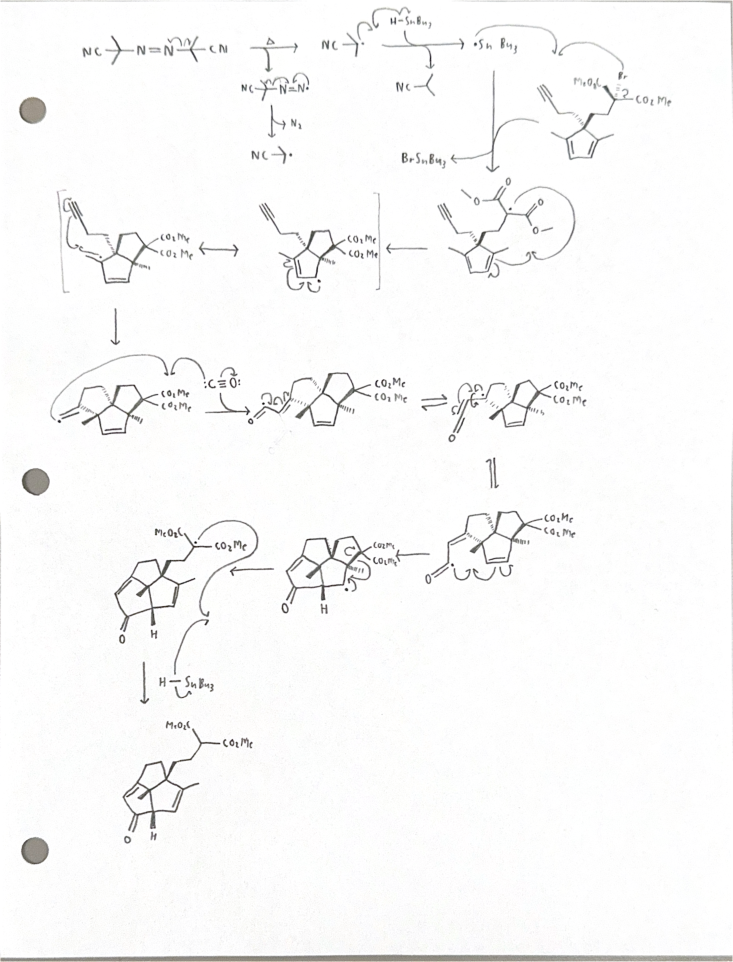
\includepdf{ExtFiles/PSet1Q1Full.pdf}
    \item We now begin discussing Problem 2.
    \begin{figure}[h!]
        \centering
        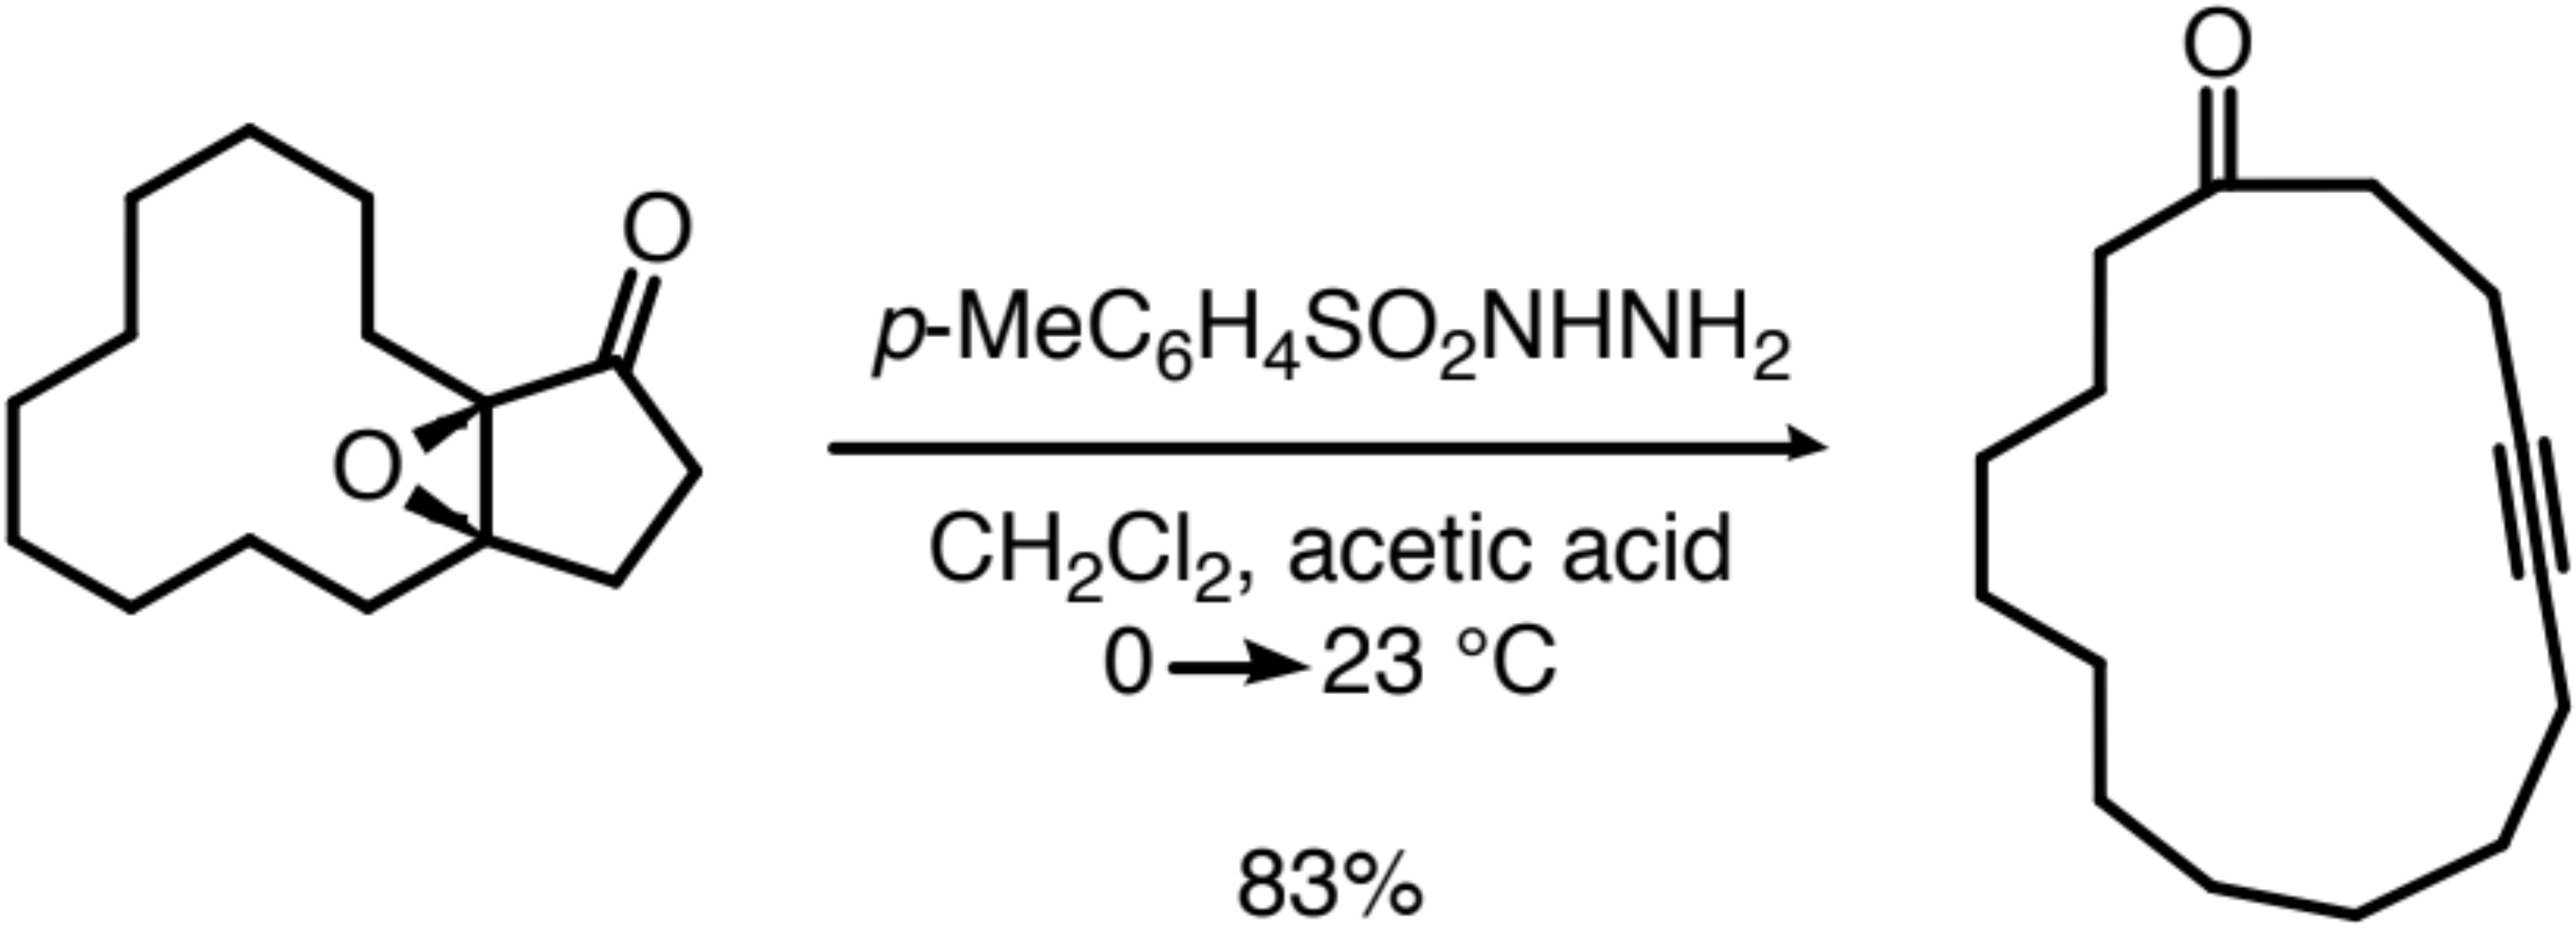
\includegraphics[width=0.5\linewidth]{PSet1Q2.png}
        \caption{PSet 1, Q2.}
        \label{fig:PSet1Q2}
    \end{figure}
    \item Aside: The naming of the reagent.
    \begin{figure}[h!]
        \centering
        \footnotesize
        \begin{subfigure}[b]{0.2\linewidth}
            \centering
            \chemfig{R-S(=[2]O)(=[6]O)-OH}
            \caption{Sulfonic acid.}
            \label{fig:sulfurOxidationa}
        \end{subfigure}
        \begin{subfigure}[b]{0.2\linewidth}
            \centering
            \chemfig{R-\charge{-90=\:}{S}(=[2]O)(=[6,,,,opacity=0]\phantom{O})-OH}
            \caption{Sulfinic acid.}
            \label{fig:sulfurOxidationb}
        \end{subfigure}
        \begin{subfigure}[b]{0.2\linewidth}
            \centering
            \chemfig{R-\charge{-90=\:,90=\:}{S}(=[6,,,,opacity=0]\phantom{O})-OH}
            \caption{Sulfenic acid.}
            \label{fig:sulfurOxidationc}
        \end{subfigure}
        \begin{subfigure}[b]{0.2\linewidth}
            \centering
            \chemfig{R-\charge{-90=\:,90=\:}{S}(=[6,,,,opacity=0]\phantom{O})-H}
            \caption{Thiol.}
            \label{fig:sulfurOxidationd}
        \end{subfigure}
        \caption{The oxidation states of sulfur.}
        \label{fig:sulfurOxidation}
    \end{figure}
    \begin{itemize}
        \item There are four different oxidation states of sulfur.
        \item They are referred to as (from most oxidized to most reduced) \textbf{sulfonic acid}, \textbf{sulfinic acid}, \textbf{sulfenic acid}, and \textbf{thiol}.
    \end{itemize}
    \item Now back to the problem at hand.
    \item In acidic solution, the first thing we can do is make the carbonyl more reactive via protonation.
    \begin{itemize}
        \item Note that the hydrazide may get protonated with the acid (and perhaps 90\% of it will be!), which would shut down nucleophilicity.
        \item But whatever hydrazide remains can do the demonstrated chemistry.
    \end{itemize}
    \item Then our hydrazine species can come in and add via nucleophilic addition.
    \item After this, we're fairly stable. But a negatively charged oxygen (like the epoxide) in acidic species can be protonated!
    \item After protonation, we'll want to break the epoxide ring. But where can we draw the electron density from?
    \begin{itemize}
        \item Looking around, notice that the second hydrazine nitrogen has a lone pair that can be used!
        \item Additionally, we can start building toward our alkyne located three carbons away from the position that could become the ketone after our new alcohol undergoes some modification.
    \end{itemize}
    \item Specifically, that modification will be kicking down the oxygen electrons to form the triple bond, kick out the leaving group, and break the leaving group in half all in one concerted step. This bond breaking process is still favorable because\dots
    \begin{itemize}
        \item The relevant orbitals align in an \textbf{antiperiplanar} fashion;
        \item We are strengthening and weakening consecutive bonds;
        \item Antibonding molecular orbitals receive donations of electron density, specifically the $\sigma^*$-antibonding orbital of the \ce{S-N} bond;
        \item The entropic gain in going from one molecule to three favors this step thermodynamically.
    \end{itemize}
    \item Aside: 4-membered transition states.
    \begin{figure}[H]
        \centering
        \footnotesize
        \schemestart
            \chemfig[atom sep=2.8em]{[:30]*6((-[:-100,0.7]!{wave})(-[:-140,0.7]!{wave})-[@{B1}]\charge{[extra sep=4pt]20=$\oplus$}{N}(-[:-40,0.7]H)(-[:-80,0.7]R)-[@{B2}]H-[@{B3},,,,opacity=0]O(-[,0.7]R)-[@{B4}]H-[@{B5},,,,opacity=0]HO-[@{B6}])}
        \schemestop
        \chemmove{
            \draw [curved arrow={2pt}{2pt}] (B6) to[bend right=40,looseness=1.2] (B5);
            \draw [curved arrow={2pt}{2pt}] (B4) to[bend right=40,looseness=1.2] (B3);
            \draw [curved arrow={2pt}{2pt}] (B2) to[bend right=40,looseness=1.2] (B1);
        }
        \caption{Using an acid as a proton transfer agent.}
        \label{fig:acidProtonTransfer}
    \end{figure}
    \begin{itemize}
        \item At a minimum, look to add an \ce{O-H} to the ring to make it a six-membered transition state.
        \item We could also do this in a two-step intermolecular process.
        \item As a specific example, amide bond hydrolysis under basic conditions is more reminiscent of the six-membered ring, though.
    \end{itemize}
    \item Aside: Protonation and $\pKa$'s.
    \begin{itemize}
        \item Ketones are much harder to protonate than comparable species.
        \begin{itemize}
            \item $\pKa$ of hydronium is $-1.7$.
            \item $\pKa$ of protonated ethylene oxide (the simplest epoxide) is $-2$.
            \item $\pKa$ of protonated carbonyl is $-6$ to $-8$.
        \end{itemize}
        \item Protonated THF is more easily stabilized by solvation effects than protonated diethyl ether because the "arms" are being held back in THF, so the oxygen lone pairs are more accessible.
        \item Carboxylic acid derivatives vary in terms of how hard they are to protonate.
        \begin{itemize}
            \item Acid chloride is $-9$.
            \item Amide is $0$ (resonance stabilization of the positive charge to the nitrogen).
            \item Ether is in the middle (still has resonance stabilization, but oxygen is more electronegative).
        \end{itemize}
    \end{itemize}
    \item Random note: Strain for a 5-membered ring is about \SI{5}{\kilo\calorie\per\mole}.
    \item Altogether, the full solution to PSet 1, Q2 is on the next page.
    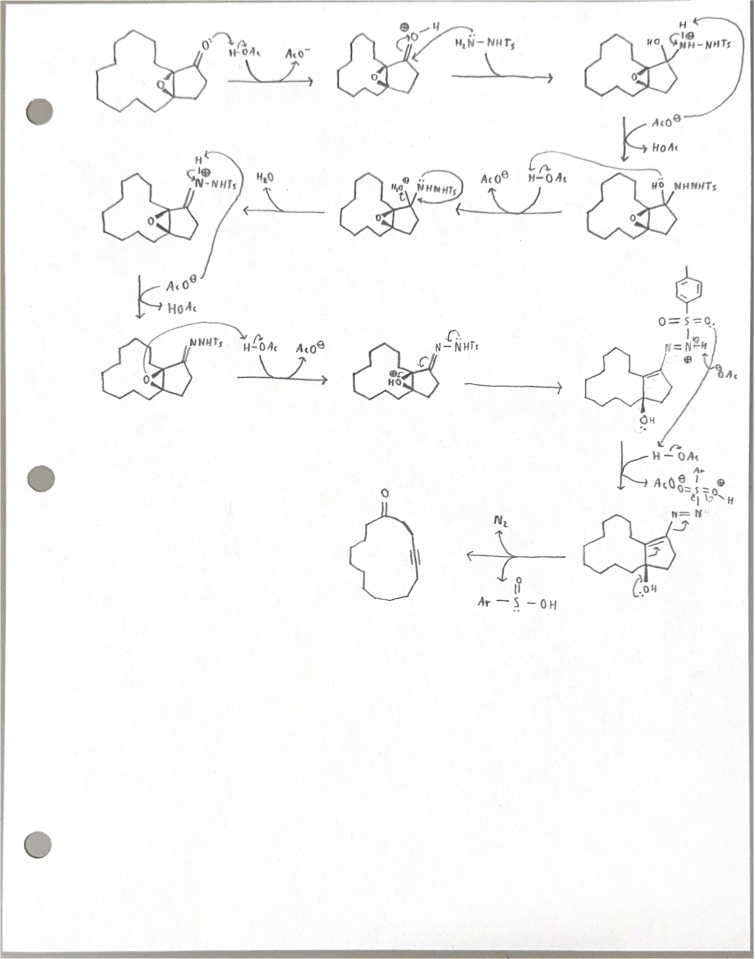
\includepdf{ExtFiles/PSet1Q2Full.pdf}
    \item We now begin discussing Problem 6.
    \begin{figure}[h!]
        \centering
        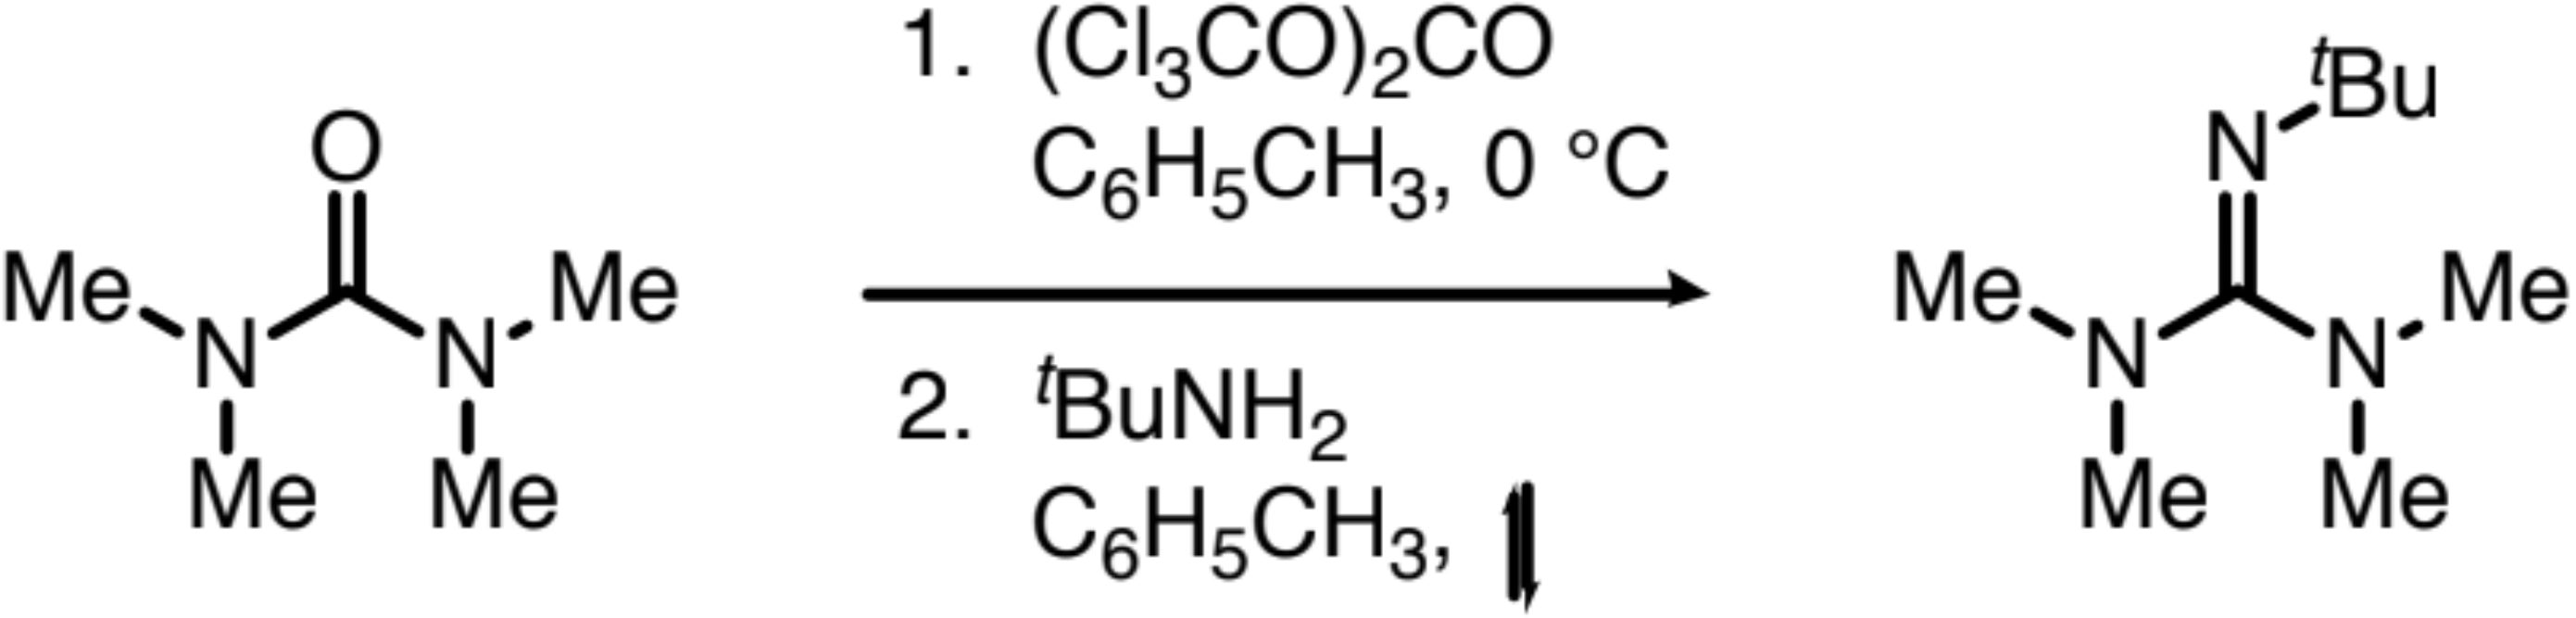
\includegraphics[width=0.5\linewidth]{PSet1Q6.png}
        \caption{PSet 1, Q6.}
        \label{fig:PSet1Q6}
    \end{figure}
    \item The first reagent is triphosgene. We use it because...
    \begin{itemize}
        \item It is far less toxic than phosgene;
        \item It generates phosgene \emph{in situ}.
    \end{itemize}
    \item First, make the reactant more nucleophilic via resonance.
    \item The reactant then attacks the reagent.
    \begin{itemize}
        \item Note that Mo is fine with us drawing out a nucleophilic substitution as electrons kicking up and back down in one step instead of in two (as Levin required). As such, I have done a bit of both in the final mechanism for this problem.
    \end{itemize}
    \item The leaving group is unstable, and undergoes $\alpha$-elimination of one chlorine.
    \item Chloride then attacks the positive center, kicking electrons up and down and kicking out a leaving group.
    \item \ce{CO2} then leaves, and we get another phosgene and chloiride.
    \item The chloride salt is where we end (the boxed intermediate in the final mechanism).
    \begin{itemize}
        \item Note that overall at this point, we've generated 2 equivalents of phosgene and 1 equivalent of \ce{CO2}; all chloride generated has been reincorporated into the molecule.
    \end{itemize}
    \item Now we add the second species.
    \item It attacks the iminium ion and kicks out the chloride.
    \item Chloride then neutralizes the molecule, generating \ce{HCl}.
    \item Finally, one more chloride attacks the remaining nitrogen hydrogen.
    \begin{itemize}
        \item Decide which way we go based on the $\pKa$'s of the relevant acids.
    \end{itemize}
    \item Note that we need one extra equivalent of \emph{tert}-butylamine to sequester the \ce{HCl}.
    \item Altogether, the full solution to PSet 1, Q6 is on the next page.
    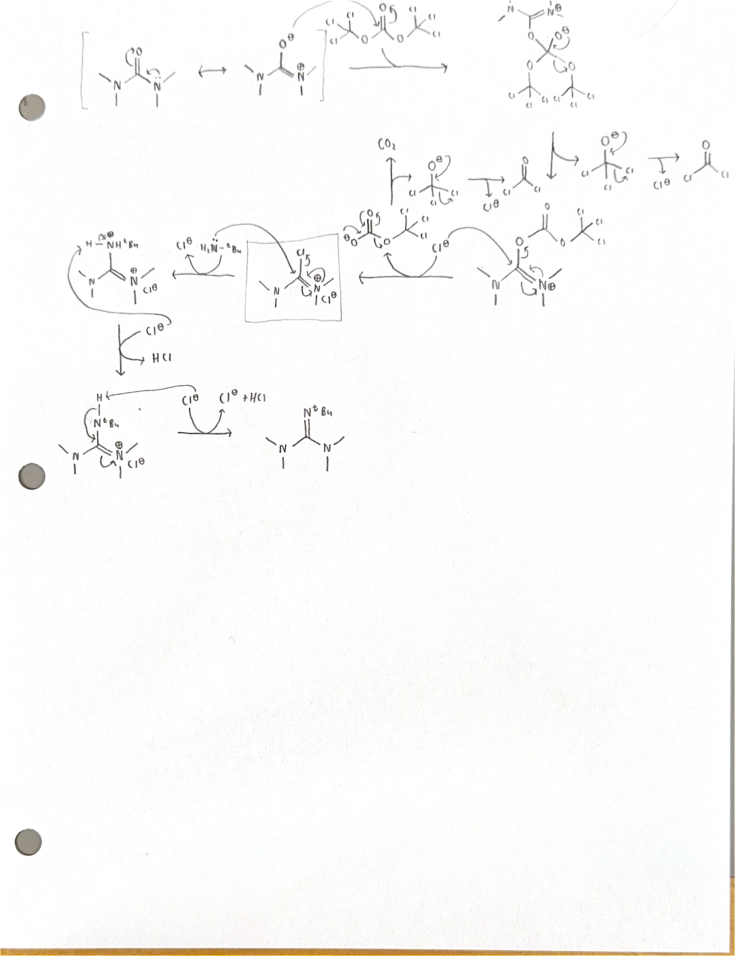
\includepdf{ExtFiles/PSet1Q6Full.pdf}
    \item Next time.
    \begin{itemize}
        \item We'll start next time with problems 4-5 of PSet 1.
        \item First 5 sessions are with Mo, then Alison has 6-10.
        \item 10 total sessions in this class.
    \end{itemize}
    \item Memorize more $\pKa$'s!!
\end{itemize}



\section{Problems 3, 4, and 5}
\begin{itemize}
    \item \marginnote{9/6:}PSet 2 PDF, please?
    \begin{itemize}
        \item Mo sent PSets 2-3 via email a minute before class.
        \item We will work all the PSets in order, as opposed to mixing and matching problems.
    \end{itemize}
    \item Mo: Prioritize working on new problems instead of clean copying old problems.
    \item We now begin discussing Problem 5.
    \begin{figure}[h!]
        \centering
        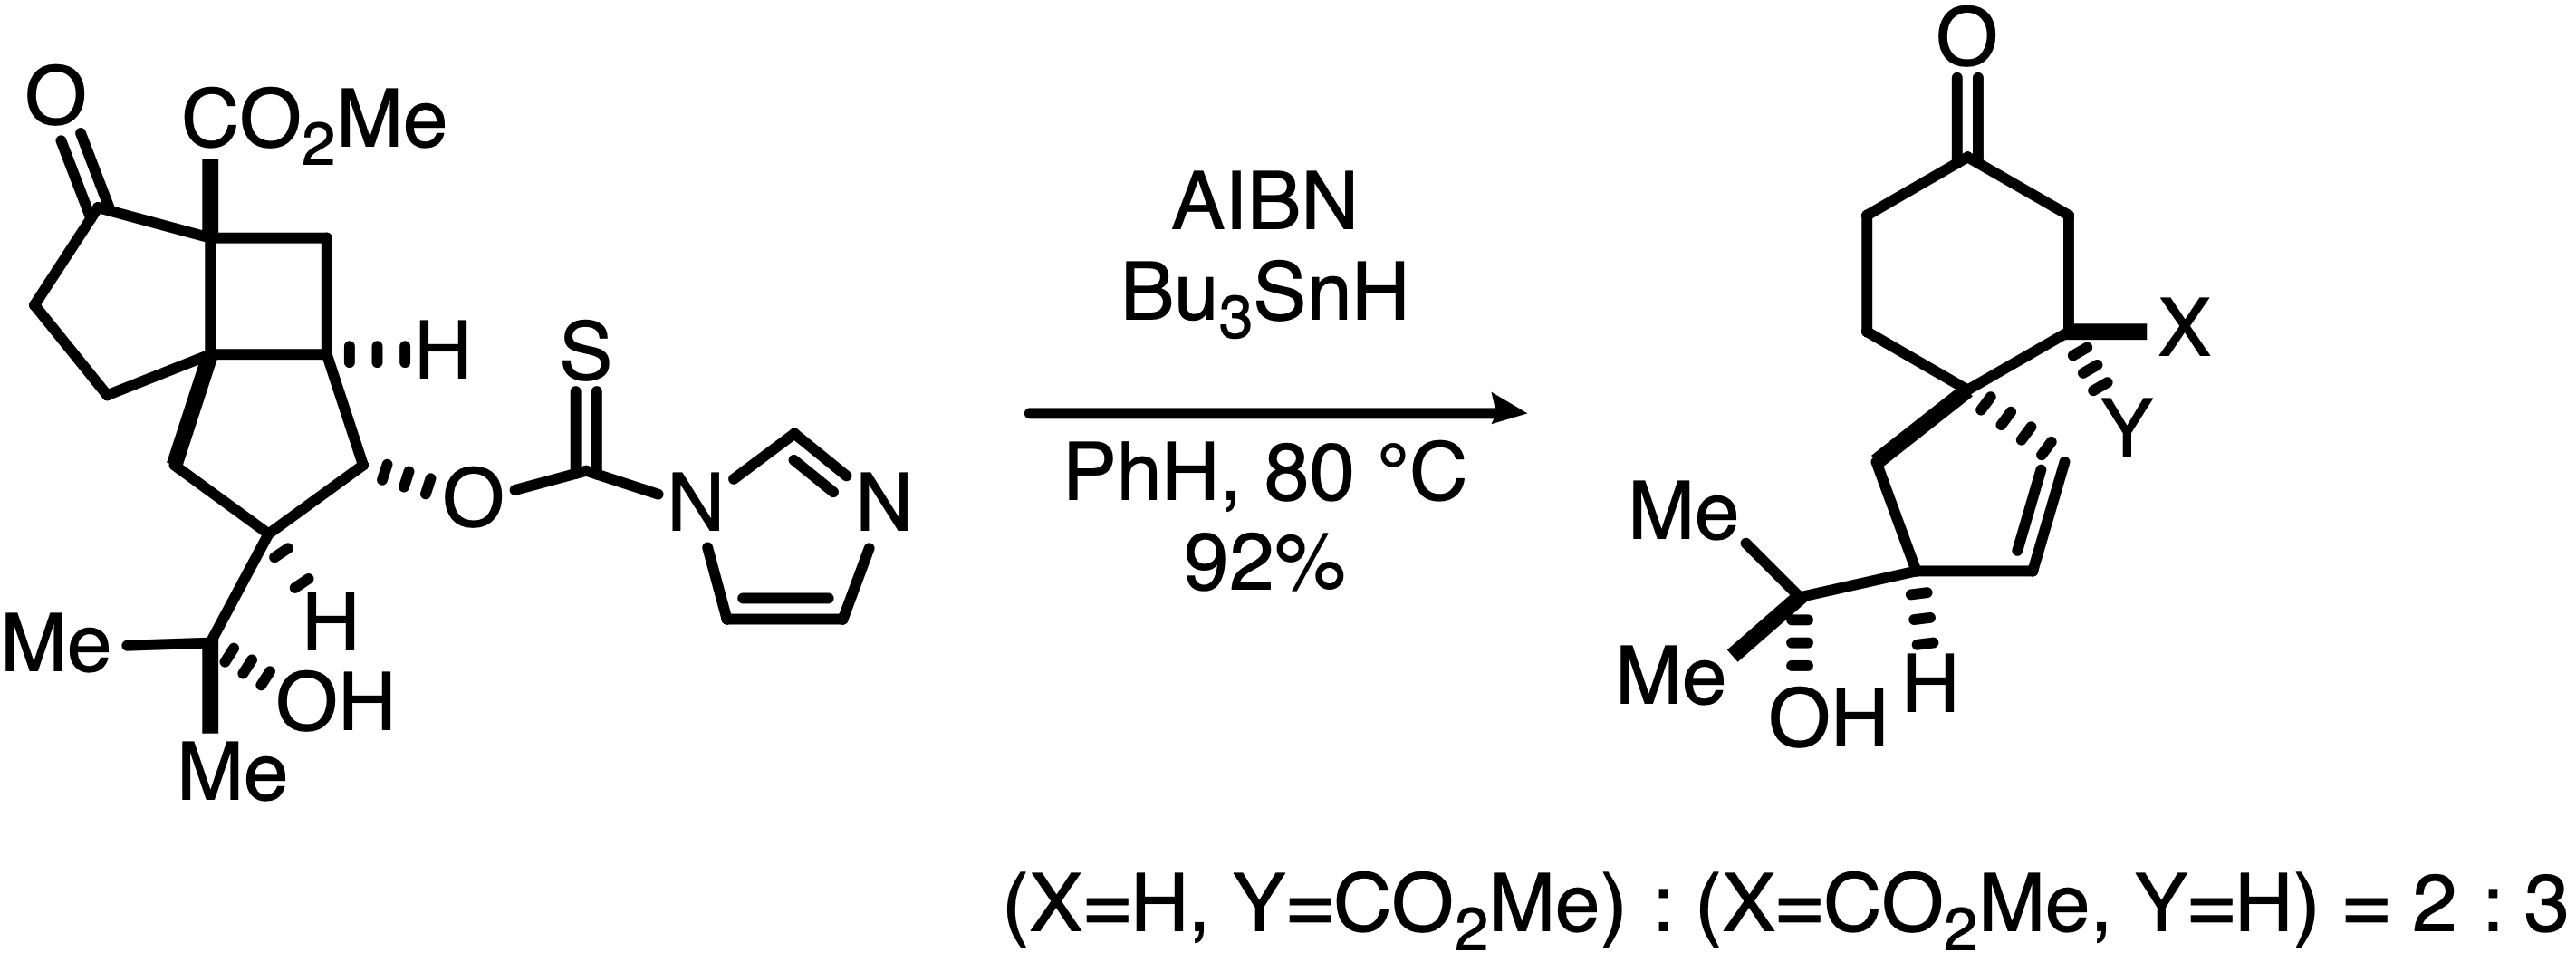
\includegraphics[width=0.55\linewidth]{PSet1Q5.png}
        \caption{PSet 1, Q5.}
        \label{fig:PSet1Q5}
    \end{figure}
    \item As in PSet 1, Q1 (Figure \ref{fig:PSet1Q1}), we start by cleaving AIBN and abstracting the hydride from \ce{HSnBu3}.
    \item Then like we went after the bromine last time, we go after the sulfur this time. Let's discuss the driving force to go after the sulfur.
    \begin{itemize}
        \item The sulfur atom, itself, is a big soft atom with orbitals that are easily accessible to the tin radical.
        \item The product is also extremely stable for several reasons.
        \begin{itemize}
            \item For starters, it's a tertiary radical.
            \item It's also a 5-electron, 3-centered radical once you take the oxygen and the sulfur into account.\footnote{Aside: This is why the methine \ce{C-H} bonds in THF are weaker than the other ones, i.e., because breaking one of them generates a 3-electron, 2-centered radical.} Essentially, all of the nearby heteroatoms can donate in electron density to stabilize the radical.
        \end{itemize}
        \item Note that among the nearby heteroatoms, the nitrogen is least likely to donate its electron pair. This is because its electron pair is part of the aromatic ring. Thus, to donate it, you would have to break aromaticity, and that would be extremely unfavorable.
    \end{itemize}
    \item Next, you kick out the whole sulfur-containing moiety as a leaving group and form a secondary radical on the compound.
    \begin{itemize}
        \item It's not immediately obvious why this step should be favorable: You're breaking a (very strong) \ce{C-O} single bond. However, you are also forming a \ce{C=O} double bond, and it's this bond-forming process which provides the driving force to split off the leaving group.
    \end{itemize}
    \item Aside: The last two steps together are known as a \textbf{Barton-McCombie deoxygenation}.
    \begin{itemize}
        \item This method works really well for tertiary alcohols.
        \item However, if you just have a primary alcohol, you will reduce the stable radical with tin hydride because it is not favorable to form a primary radical. Then under acidic work up conditions, you kick out the alcohol from the thioester.
    \end{itemize}
    \item Once again, it is now not immediately obvious how to proceed.
    \begin{itemize}
        \item We can't really have a 5-endo-trig cyclization (under ordinary OChem conditions).
        \item One thing we can do is form the double bond in the product, break a \ce{C-C} $\sigma$-bond, and form a methyl radical.
        \item This seems like it would be very uphill at first, but it will be driven by the release of the cyclobutane ring strain. Indeed, so much strain release is the only thing that could drive primary radical formation.
    \end{itemize}
    \item Then we have a 3-exo-trig cyclization.
    \begin{itemize}
        \item This is a kinetically favorable (but reversible) cyclization.
        \item It is also favorable because it eliminates the primary radical.
        \item Radicals abstract atoms that have spherical orbitals (I, Br, Cl, H).
        \begin{itemize}
            \item Radicals don't abstract methyl groups because it would have to invert the carbon atom and navigate the \ce{C-H} orbitals to get to the \ce{C-C} $\sigma^*$ orbital.
            \item Adding into the \ce{C=O} $\pi$-bond is just gonna be more favorable, even though we're forming a 3-membered ring.
        \end{itemize}
        \item How fast is the formation of the three-membered ring?
        \begin{itemize}
            \item Going to a primary oxygen centered radical is uphill.
            \item Exchanging a $\pi$-bond for a \ce{C-C} $\sigma$-bond is favorable.
            \item We are also helped by the fact that fragmentation is very exothermic, so even though we have to go through a high-energy intermediate, we get a very stable product one step later. In fact, the energetic stability of the product \emph{lowers} the energy of the transition state (and hence the activation energy).
        \end{itemize}
        \item Know rates, too!!
        \begin{itemize}
            \item Releasing ring strain in the radical clock radical is \SI{e8}{\per\second}.
            \item 5-exo-trig is \SI{e5}{\per\second}.
            \item Radical-radical coupling is almost barrierless; diffusion controlled at \SI{e9}{\per\second}.
            \item Going from the strained, primary radical to a doubly benzylic radical can happen faster than diffusion at \SI{e11}{\per\second}.
            \item Relearn radical clocks!!
        \end{itemize}
    \end{itemize}
    \item Because the 3-exo-trig is reversible, we could just reverse it. However, there is another, more favorable route.
    \begin{itemize}
        \item Indeed, the last step is driven by the release of cyclopropane ring strain and the formation of a tertiary, resonance-stabilized radical.
    \end{itemize}
    \item We get a rearrangement and fragmentation.
    \item The spiro group and sterics could account for the ratio of stereoisomers.
    \begin{itemize}
        \item Alkene vs. alkane already favors the stereochemistry; we don't \emph{need} the \ce{R} group. The alkene is so much smaller (2 hydrogens vs. 4 hydrogens).
    \end{itemize}
    \item Altogether, the full solution to PSet 1, Q5 is on the next page.
    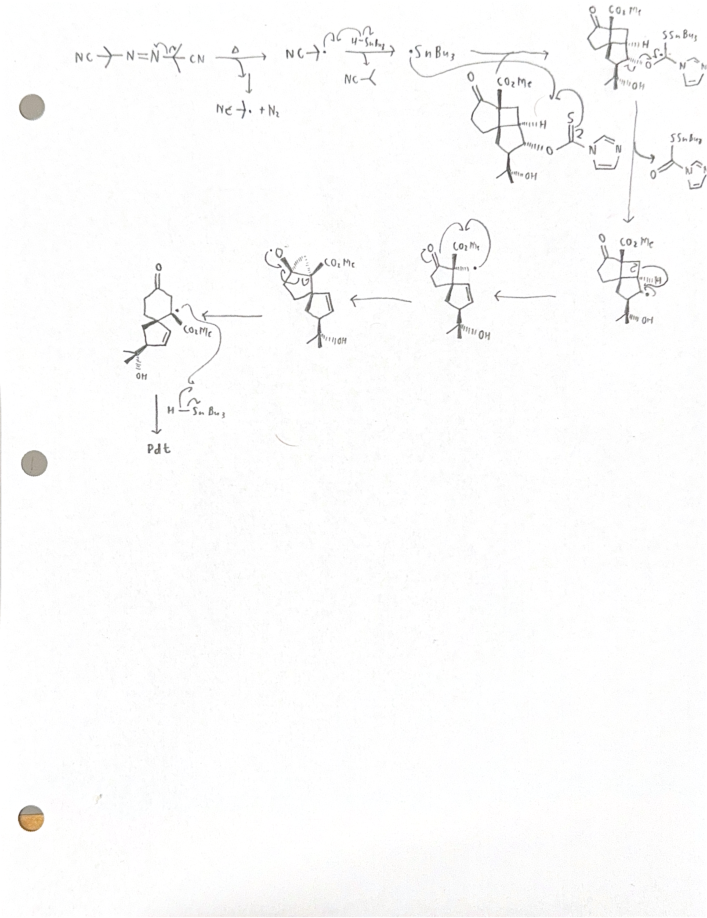
\includepdf{ExtFiles/PSet1Q5Full.pdf}
    \item We now begin discussing Problem 4.
    \begin{figure}[h!]
        \centering
        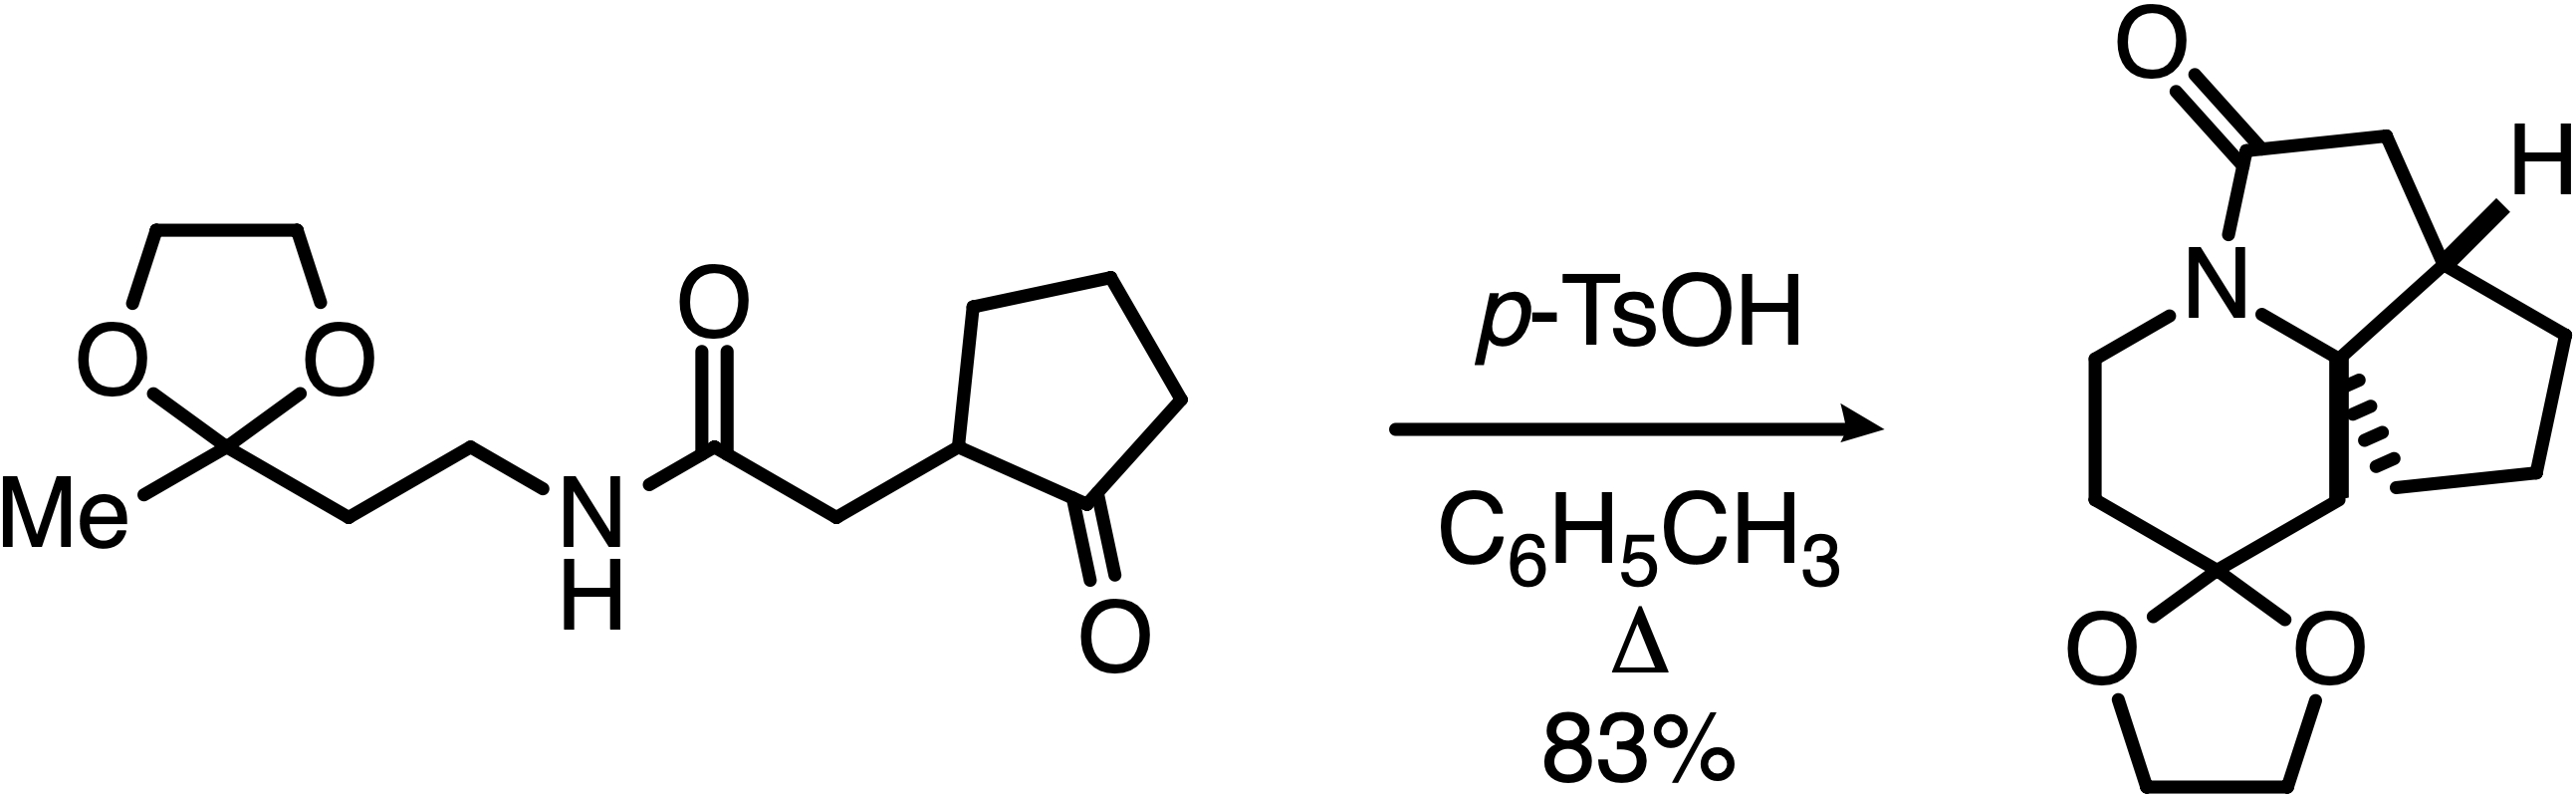
\includegraphics[width=0.45\linewidth]{PSet1Q4.png}
        \caption{PSet 1, Q4.}
        \label{fig:PSet1Q4}
    \end{figure}
    \item The provided reagents are strong acid and heat. As such, the first step will be a protonation. But which site will we protonate?
    \begin{itemize}
        \item There are five possible positions we could protonate, and four distinct types. Let's order them from least-likely to most-likely to be protonated.
        \begin{enumerate}
            \item Least likely: The amide nitrogen.
            \begin{itemize}
                \item This nitrogen's lone pair is conjugated with the \ce{C=O} $\pi$-bond, and breaking this conjugation will take a ton of energy.
            \end{itemize}
            \item The ketone.
            \begin{itemize}
                \item Recall that the $\pKa$ of a protonated carbonyl is $-6$ to $-8$.
            \end{itemize}
            \item Either of the ethers.
            \begin{itemize}
                \item Recall that the $\pKa$ of a protonated ether is $-2$.
            \end{itemize}
            \item The amide oxygen.
            \begin{itemize}
                \item Recall that the $\pKa$ of a protonated amide is $0$.
                \item This is because the positive charge we create is resonance-stabilized by the $\alpha$-nitrogen.
            \end{itemize}
        \end{enumerate}
        \item Thus, while protonating the ketone would seem like a logical first step to accelerate nucleophilic addition, he $\pKa$ values tell us that it is \emph{over a million times} more likely that we will protonate the amide first.
        \item Moreover, this protonation actually is helpful!
        \begin{itemize}
            \item Specifically, it can help tautomerize the amide into an \textbf{imidic acid}.
            \item The imidic acid's nitrogen will then have an unconjugated lone pair in an $sp^2$ orbital that is ideally positioned to attack the ketone once we protonate it. This imidic acid/\textbf{imidate}\footnote{Clear up the naming!} nitrogen is a superb nucleophile.
        \end{itemize}
    \end{itemize}
    \item Thus, after the tautomerization, we activate the ketone and add into it.
    \begin{itemize}
        \item This forms a fairly stable hemiaminal that can hang around for a while.
        \item In particular, we will \emph{not} want to convert this to an \ce{N}-acyliminium just yet (see below).
    \end{itemize}
    \item We then deprotonate the intermediate so that we can protonate it elsewhere.
    \begin{itemize}
        \item It is important to deprotonate \emph{before} charging ahead into the next protonation because multiply charged intermediates are difficult to access.
    \end{itemize}
    \item Once we activate the ketal, multiple species in solution could pick off the $\alpha$-hydrogen.
    \begin{itemize}
        \item It could be the conjugate base, tosylate. However, it could also be the original amide in the starting material!
    \end{itemize}
    \item At this point, our enol ether is a prepared and ready nucleophile.
    \item Now we activate the electrophile by having water leave to create an \ce{N}-acyliminium.
    \begin{itemize}
        \item \ce{N}-acyliminiums are even more electrophilic than iminiums due to their combined dipole with the adjacent carbonyl.
        \item Thus, it is important that we form the enol ether first and the \ce{N}-acyliminium second, because the \ce{N}-acyliminium will react as soon as it forms. In other words, the \ce{N}-acyliminium will not want to hang around for too many steps before reacting again.
    \end{itemize}
    \item The last step is a 5-endo cyclization, which is not feasible in radical chemistry but \emph{is} feasible in carbocation chemistry.\footnote{Is it not a 6-endo cyclization??}
    \item Comment: When working in acidic regimes, try not to have carbanions in your mechanism.
    \item This whole transformation is related to the \textbf{Pictet-Spengler reaction}.
    \item Altogether, the full solution to PSet 1, Q4 is on the next page.
    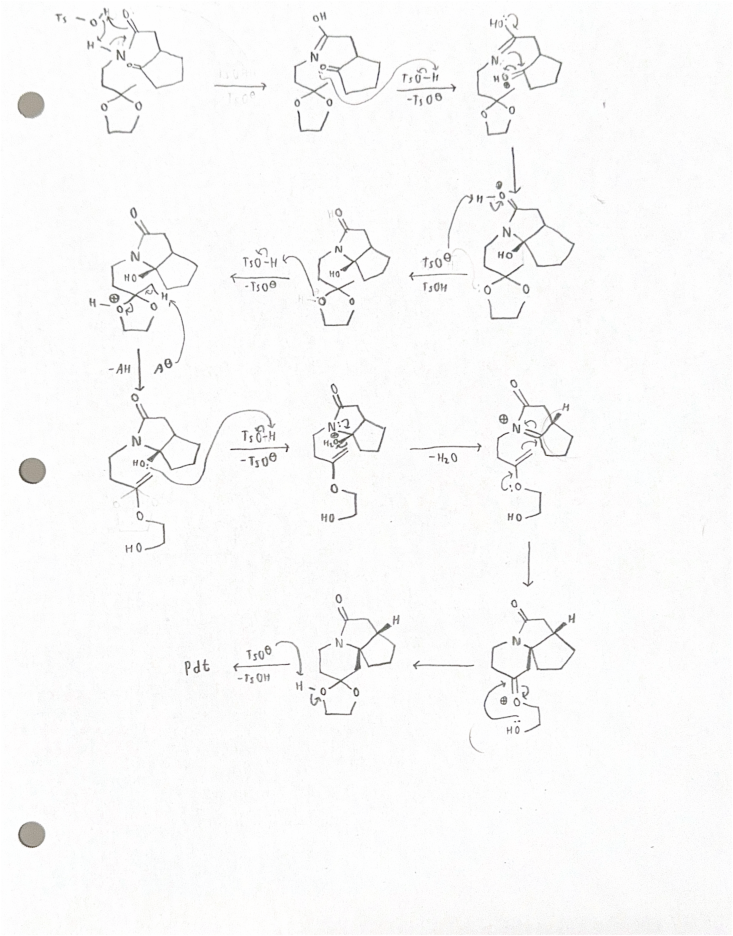
\includepdf{ExtFiles/PSet1Q4Full.pdf}
    \item We now begin discussing Problem 3.
    \begin{figure}[h!]
        \centering
        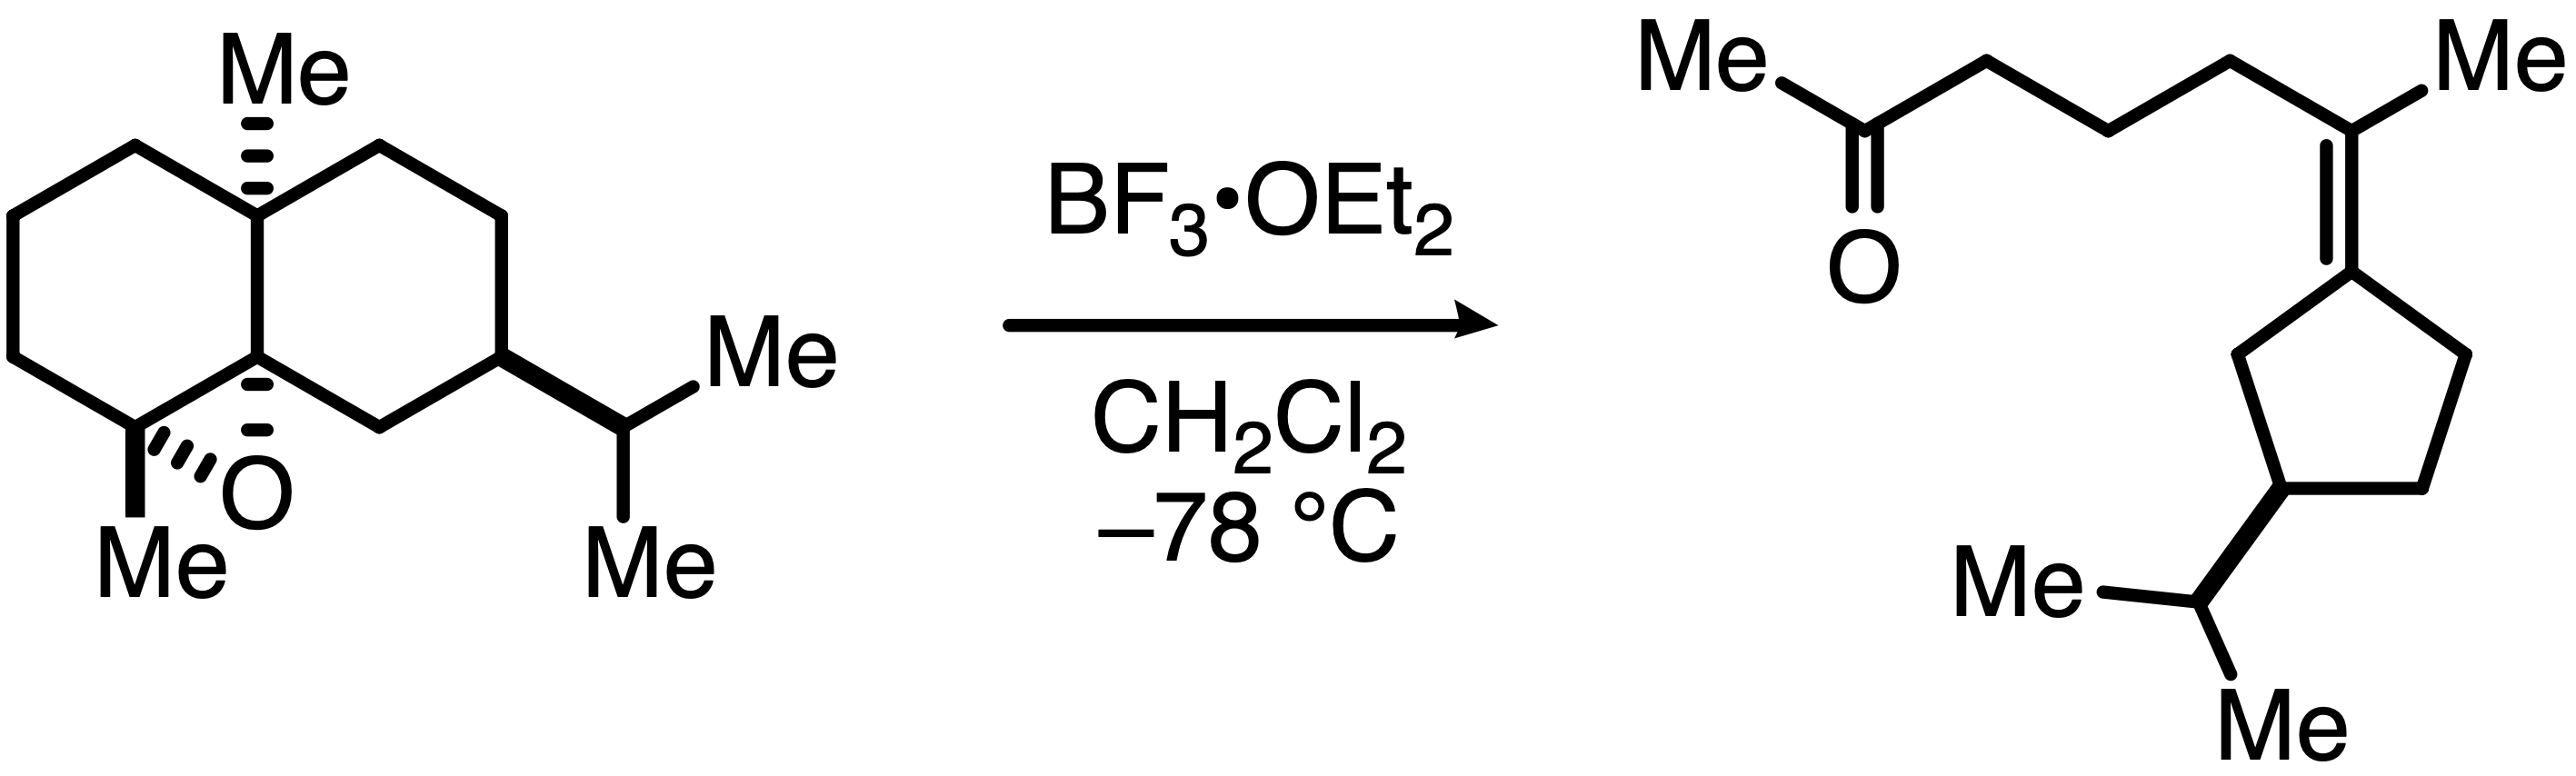
\includegraphics[width=0.45\linewidth]{PSet1Q3.png}
        \caption{PSet 1, Q3.}
        \label{fig:PSet1Q3}
    \end{figure}
    \item Looking at the reagents, observe that \ce{BF3} is a strong Lewis acid. Thus, it will seek out the most nucleophilic site on the substrate first, which in this case happens to be oxygen.
    \begin{itemize}
        \item When the oxygen coordinates to the boron, a number of subtle changes begin to take place.
        \item For starters, the two \ce{C-O} bonds will elongate because oxygen withdraws electron density from them. This lowers the activation energy for \ce{C-O} bond cleavage.
        \item Additionally, when oxygen has a positive charge, it becomes more electronegative and puts partial positive charges on the \textbf{distal} carbons. This makes them more promising electrophilic sites.
    \end{itemize}
    \item Drawn toward the electrophilic distal carbon, a \ce{C-C} $\sigma$-bond engages the \ce{C-O} $\sigma^*$-orbital in an antiperiplanar fashion.
    \begin{itemize}
        \item Geometry is important here: If the stereochemistry were switched at the top carbon, this reaction would be much less likely to proceed.
        \item It is also important to note that epoxide opening and ring shrinking happen in a concerted step --- driven by the favorable bonding/antibonding interactions --- instead of in a stepwise fashion.
        \begin{itemize}
            \item Indeed, antiperiplanar geometry and concerted steps often go hand-in-hand!
        \end{itemize}
        \item We can also rationalize why we have an intramolecular nucleophilic attack on the \ce{C-O} bond instead of an intermolecular one. This mainly comes down to sterics: Nucleophilic addition will be disfavored at a quaternary carbon.
    \end{itemize}
    \item At this point, we have a tertiary carbocation as our most reactive site.
    \begin{itemize}
        \item This could induce a hydride shift, but a hydride shift would form a secondary carbocation and hence this is disfavored. The only time that a hydride shift would happen here is if we could get to a much more stable product through this hydride shift.
        \item There is also no methyl shift here because the methyl group is \emph{syn}; if it were \emph{trans}, it could benefit from antiperiplanar interactions and would be more likely to shift. What does this mean??
    \end{itemize}
    \item Thus, we kick off the leaving group, form a \ce{C=O} bond and a \ce{C=C} bond, and neutralize the carbocation. All of these favorable effects are enough to compensate for breaking the \ce{C-C} $\sigma$-bond.
    \item Altogether, the full solution to PSet 1, Q3 is on the next page.
    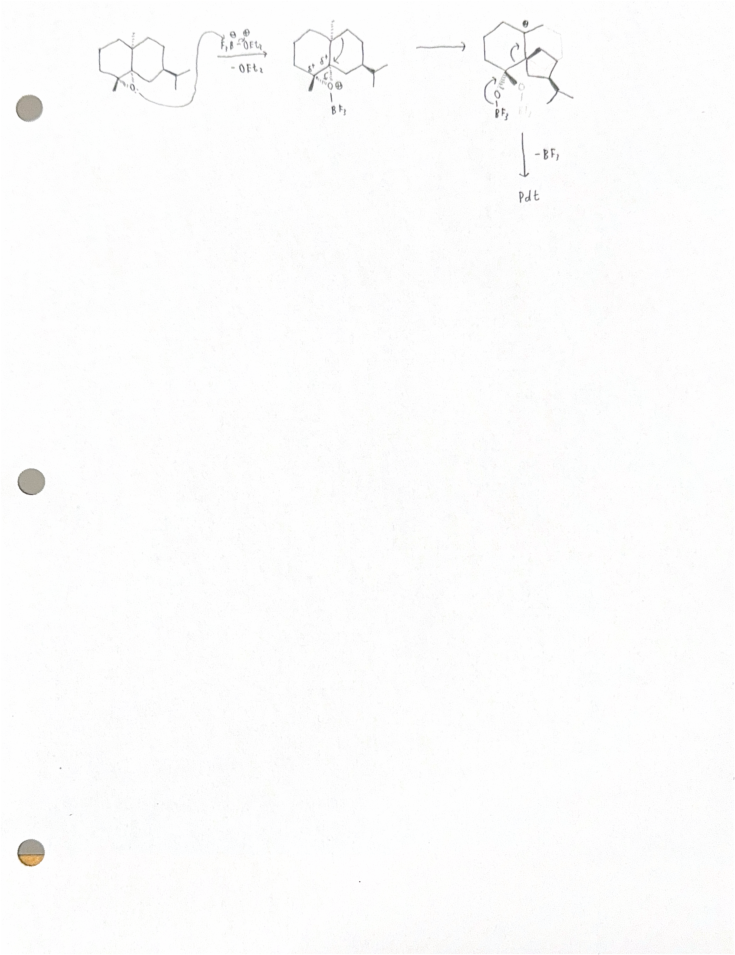
\includepdf{ExtFiles/PSet1Q3Full.pdf}
\end{itemize}




\end{document}